%%%%% Document Setup %%%%%%%%

\documentclass[10pt, twocolumn]{revtex4}    % Font size (10,11 or 12pt) and column number (one or two).

\usepackage{times}                          % Times New Roman font type

\usepackage[a4paper, left=1.85cm, right=1.85cm,
 top=1.85cm, bottom=1.85cm]{geometry}       % Defines paper size and margin length

\usepackage[font=small,
labelfont=bf]{caption}                      % Defines caption font size as 9pt and caption title bolded


\usepackage{graphics,graphicx,epsfig,ulem}	% Makes sure all graphics works
\usepackage{amsmath} 						% Adds mathematical features for equations

\DeclareMathOperator{\sech}{sech}		% Defining sech so it doesn't italicise it 
\DeclareMathOperator{\Int}{Int}		% Defining 'integer part of' so it doesn't italicise it 
\providecommand{\e}[1]{\ensuremath{\times 10^{#1}}} %shorthand for scientific notation

\usepackage{etoolbox}                       % Customise date to preferred format
\makeatletter
\patchcmd{\frontmatter@RRAP@format}{(}{}{}{}
\patchcmd{\frontmatter@RRAP@format}{)}{}{}{}
\renewcommand\Dated@name{}
\makeatother

\usepackage{fancyhdr}


\pagestyle{fancy}                           % Insert header
\renewcommand{\headrulewidth}{0pt}
\lhead{L. P. Flower}                          % Your name
\rhead{Collisions of Matter-Wave Solitons in a Bose-Einstein Condensate}            % Your report title               

\def\bibsection{\section*{References}}        % Position reference section correctly


%%%%% Document %%%%%
\begin{document}                     


\title{Collisions of Matter-Wave Solitons in a Bose-Einstein Condensate} 
\date{Submitted: \today{}}
\author{L. P. Flower}
\affiliation{\normalfont Durham University L3 Computing Project}

\begin{abstract}              
 
ABSTRACT ABSTRACT ABSTRACT ABSTRACT ABSTRACT ABSTRACT ABSTRACT ABSTRACT ABSTRACT ABSTRACT ABSTRACT ABSTRACT ABSTRACT ABSTRACT ABSTRACT ABSTRACT ABSTRACT ABSTRACT ABSTRACT ABSTRACT ABSTRACT ABSTRACT ABSTRACT ABSTRACT ABSTRACT ABSTRACT ABSTRACT ABSTRACT ABSTRACT ABSTRACT ABSTRACT ABSTRACT ABSTRACT ABSTRACT ABSTRACT ABSTRACT ABSTRACT ABSTRACT ABSTRACT ABSTRACT 

\end{abstract}

\maketitle
\thispagestyle{plain} % produces page number for front page


%%%%%%%%%%%%%%%%%%%%%%%%%%%

\section{Introduction and Theory} \label{Intro}

Solitary waves or solitons occur in systems where non-linear effects exactly cancel the dispersion of a wave packet, meaning it propagates without changing its shape. Even after collisions with other solitons, these waves emerge with their velocities and shapes unchanged, though a phase shift is imparted to both solitons. Non-linear wave systems are found in water waves, optical fibres and atomic Bose-Einstein condensates (BECs). The latter are described to a good approximation by the non-linear Schr\"{o}dinger equation when the radial confinement of the BEC is good enough that the motion is approximately one-dimensional. 

To describe the behaviour of a Bose-Einstein condensate, an effective potential term $g |\psi|^2$  is introduced into the Schr\"{o}dinger equation to characterise the interactions between the constituent particles. The resulting non-linear Schr\"{o}dinger equation is given by 
\begin{equation} \label{NLSE}
i \hbar \frac{\partial \psi}{\partial t} = -\frac{\hbar^2}{2m} \frac{\partial^2 \psi}{\partial x^2} + (V+g |\psi|^2) \psi,
\end{equation}
where $V$ is the external potential and $|\psi|^2$ represents the density of particles. $\psi$ is normalised such that the integral over all space gives $N$, the number of particles in the soliton system. Describing the interparticle interaction by the pseudopotential approximation $g |\psi|^2$ is valid in the dilute limit, where the average spacing between gas particles is greater than the scattering length, $a_s$. 

However, the length scales of the simulation must also be such that the individual behaviour of atoms in the solitons is not of interest. A characteristic soliton length $\xi$ can be defined such that on length scales longer than $\xi$, atoms move collectively (as a recognisable soliton) while on shorter length scales, they behave as free particles. Here the soliton length is defined as $\xi = \frac{\hbar^2}{mg}$ \cite{Cornish}. Using the transformations \cite{Transforms} 
\begin{equation} \label{transforms}
x = \tilde{x} \frac{\xi}{\sqrt{2}}, \quad		 t = \tilde{t} \frac{m \xi^2}{\hbar}, 	\quad \psi = \tilde{\psi} \frac{1}{\sqrt{\xi}}
\end{equation}
%\quad inserts quadruple space
to rescale quantities in the nonlinear Schr\"{o}dinger equation, the Gross-Pitaevskii equation (GPE) in its dimensionless form is obtained \cite{Gross} \cite{Pitaevskii}
\begin{equation} \label{GPE}
i \frac{\partial \tilde{\psi}}{\partial \tilde{t}} = -\frac{\partial^2 \tilde{\psi}}{\partial \tilde{x}^2} + (\tilde{V}+g |\tilde{\psi}|^2) \tilde{\psi},
\end{equation}
where the tilde symbols denoting the transformed quantities are omitted for the rest of this report, for clarity of reading. 

The integrable solutions to the Gross-Pitaevskii equation are $\sech$ solitons. A parameter to characterise width, $\zeta$, can be defined with units 1/length. The normalised initial wavefunction is then 
\begin{equation} \label{soliton}
\psi(x) = \sqrt{\frac{\zeta}{2}} \sech{(\zeta x)} e^{i (v x + \phi)},
\end{equation}
where $v$ is the velocity of the soliton and $\phi$ is a phase factor. In order for the soliton to propagate without change of shape, it is required that $g=-4\zeta$. This is found by substituting the $v=0$ case into the time-independent nonlinear dimensionless Schr\"{o}dinger equation and setting $E$ to be $\zeta^2$ to find the stationary-state condition. It is predicted that if the value of $g$ found to confine the soliton in this simulation differs from $-4\zeta$, it is due to the treatment of space and time as discrete variables rather than continuous. 

The solutions to the GPE come in two forms. If the interactions are repulsive, i.e. the scattering length between atoms is positive, the interaction parameter $g$ is positive and hence the solutions are 'dark solitons': atom density minima which move without changing shape. But if the interactions are attractive (negative scattering length), the solutions are bright matter-wave solitons with negative $g$, where the centre of a soliton corresponds to a maximum atomic density. In this report we will consider bright solitons only. These can be produced either with a BEC of atoms with an intrinsic negative scattering length, or by tuning the interactions using a Feshbach resonance \cite{Feshbach}. 

To check that the length scales of this simulation are suitable for modelling solitons as a collective, we express the interaction parameter $g$ in terms of the parameters of the experimental system. A Bose-Einstein condensate of Rubidium-85 atoms hs been chosen, which has an intrinsic scattering length of $a_s = -0.6$ nm and 2000 atoms per soliton \cite{ExpParams}. The radial confinement, which has been assumed to be perfect in the computational part of this project to reduce the problem to 1D, has frequency $\omega_r = 2\pi \times 17.5$ Hz. Note however that the 1D axial confinement, if present, is explicitly dealt with in this simulation. $|g| = 2\hbar \omega_r |a_s| N$ \cite{Cornish} is then equal to $2.78 \e{-38}$ kg m$^3$ s$^{-2}$. This implies $\xi = 2.82 \mu$m. A single unit of rescaled length is equivalent to $\xi/\sqrt{2} = 1.99 \mu$m and box lengths between 20 and 40 rescaled space units are used in this model, hence the length scales are suitable for modelling the behaviour of solitons. In the graphs in this report, the unit of time has also been multiplied by 10 to improve readability. The unit of time displayed on graphs is therefore equal to 0.00107 s, so the simulation was run for at least 0.0214 s and up to 0.128 s. Most experiments are run over the course of $\sim$ 35 ms, around the same order of magnitude as this computational model. 

The name 'solitons' for solitary waves originates from the fact that their dynamics are (largely) unchanged after collisions with other solitons, playing on the usual nomenclature for particles where their names end in '-on'. Throughout the history of solitons, in both water and optical systems, a classical particle model has been useful for describing their motion in applications where the details of collisions are unimportant. An interpretation (?) of the particle model for matter-wave solitons in Bose-Einstein condensates was developed recently \cite{Martin}. The particles are placed in the same external potential $V$ as the solitons, and an effective inter-soliton potential 
\begin{equation}
V(q_j - q_k) = -\eta \sech^2{\eta(q_j - q_k)}
\end{equation}
is a valid approximation when the solitons have equal effective masses $\eta$. $q_i$ is the position of soliton $i$ as a function of time. This potential does not describe the interference effects produced when solitons collide, since classical particles do not exhibit wave-like properties, so it is only a good descriptor away from collision sites. But for soliton separations greater than $2/\eta$, the attractive potential is extremely weak. As a result, if the average soliton separation is greater than $2/\eta$, the inter-soliton potential can be approximated as zero. This will not allow for the formation of bound states of particles \cite{Bound} and will have impacts on the frequency of collisions when the particles are confined in a harmonic trap. The validity of this approximation will be investigated in this project. 

%%%%%%%%%%%%%%%%%%%%%%%%%%%%%%%%%%%%%%%%%%%%%%%%%%%%%%%

\section{Methods} \label{Methods}

The split-step Fourier method is a mathematical trick borrowed from optics and relies on the fact that in Fourier space, the operator $\frac{d}{dx}$ becomes $k$, the transformed variable with units 1/length. The wavefunction is multiplied by a small nonlinear step in the form of the exponential of the potential multiplied by $\delta t$. It is then Fourier transformed and multiplied by the kinetic energy factor in terms of $k$. Once the wavefunction has been propagated in k-space, the inverse Fourier transform is taken. The wavefunction at a time $t+\delta t$ is then given by

\begin{equation} \label{fft}
\psi(x,t+\delta t) = \mathcal{F}^{-1}[e^{ik^2 \delta t} \mathcal{F} [e^{-i(V+g|\psi|^2) \delta t} \psi(x,t) ] ],
\end{equation}
where $V$, $g$ and $\psi$ are defined above in the Gross-Pitaevskii equation. 

The discrete $k$ values are found from $\delta k = \frac{1}{n \delta x}$. The Fast Fourier Transform module \texttt{numpy.fft} was used to compute the discrete Fourier tranforms and inverses. The space-time box was initially 20x20 for the purpose of obtaining preliminary results, and was increased to 40x40 for repeated collisions. Initially 2000, then 4000 space points and 4000 time points were used to minimise discretisation effects. 

An accuracy test function was written to integrate $|\psi|^2$ over a given range of $x$ and compare the initial norm to that at a time $t$. This is evaluated for the case where the soliton has zero velocity and hence is localised over the same range of $x$ throughout the simulation. The function \texttt{numpy.trapz} was used to numerically integrate using the trapezium rule, which is a good approximation as $\delta x$ was small (0.01 in the case of repeated collisions). This gives a measure of the probability leakage which occurred during propagation, which is related to the numerical limits of the split-step Fourier method and the discretisation of space and time. The $x$ limits were taken to be well within the box, to avoid discontinuity errors at the edges. 

The extension to two (or more) solitons was trivial: the initial wavefunction became a sum of the individual soliton wavefunctions. This had the effect of reducing the effective soliton mass from 1 to $1/N$ where N is the number of solitons. The only difference is that with more than one soliton, the relative phase between the solitons must be specified in the case that they collide. The phase of a soliton, while an integral part of its wave nature, does not affect its dynamics at all and is only important at the point of collision with another soliton. The first soliton was implemented with phase $\phi = 0$ in Eqn. \ref{soliton} above, and subsequent solitons were given a constant relative phase $\phi=\Delta \phi$. In this investigation, only pairs (or triples) of solitons with the same family parameter $\zeta_i=\zeta_j$ have been considered. This is realistic, since all solitons formed in a homogeneous Bose-Einstein condensate will have the same family parameter as it depends on the strength of the interactions between atoms, $g$. For simplicity, we have also only considered solitons with the same speed $|v_i| = |v_j|$. In an experiment the soliton velocities can be tuned by the experimenter. 

The idea of modelling solitons as classical particles originates in optics but was explored in matter-wave solitons by Martin et al. \cite{Martin}. In this project, the approximation of solitons as emerging completely unchanged from collisions was investigated by using a particle model with no inter-soliton potential. Particles were introduced into the same harmonic potential as the solitons and hence underwent simple harmonic motion about the centre of mass at $x=0$. For 2 solitons, the particles were each given mass 0.5 to agree with the soliton masses as described above ($1/N$ where $N=2$), so that both wave solitons and particles behaved identically in the harmonic trap. 

%%%%%%%%%%%%%%%%%%%%%%%%%%%%%%%%%%%%%%%%%%%%%%%%%%%%%%%

\section{Preliminary Results} \label{Milestone}

 For $\zeta=1$, it was found by trial and error that $g=-4$ confined the soliton, in perfect agreement with theory. The accuracy test described in Section \ref{Methods} was run over the interval $x \in (-2.5,2.5)$, giving a probability leakage of 0.009\% over the extent of the experiment, $t$ from 0 to 20. This result is within the goal of this model of keeping probability leakage under 0.01\%. 

\begin{figure}[h]
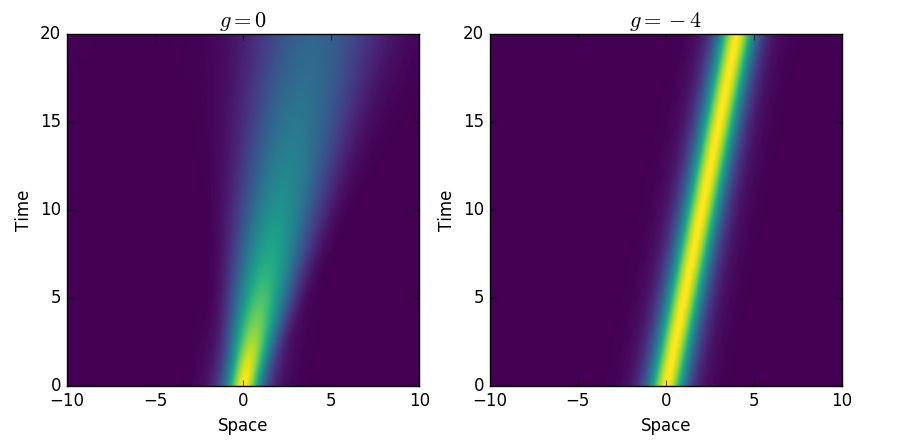
\includegraphics[width=\columnwidth]{milestonepic.png}
\caption{A graph showing the effect of inter-atom interactions $g |\psi|^2$ on a soliton model. The family 
parameter $\zeta = 1$ hence $g=-4$ perfectly confines the soliton with velocity $v=0.2$.}
\end{figure}

Since there was a small amount of probability leakage with $g=-4$, values of $g$ in a small range $\Delta g = 0.01$ either side of the theoretical value were investigated. The accuracy test was run on each, for a space-time box of 2000x2000 points ($x \in [-10,10]$, $t \in [0,2]$) and 6000x6000 points ($x \in [-10,10]$, $t \in [0,6]$). The results are plotted in Fig. \ref{errorsfig}. 

\begin{figure}[h] 
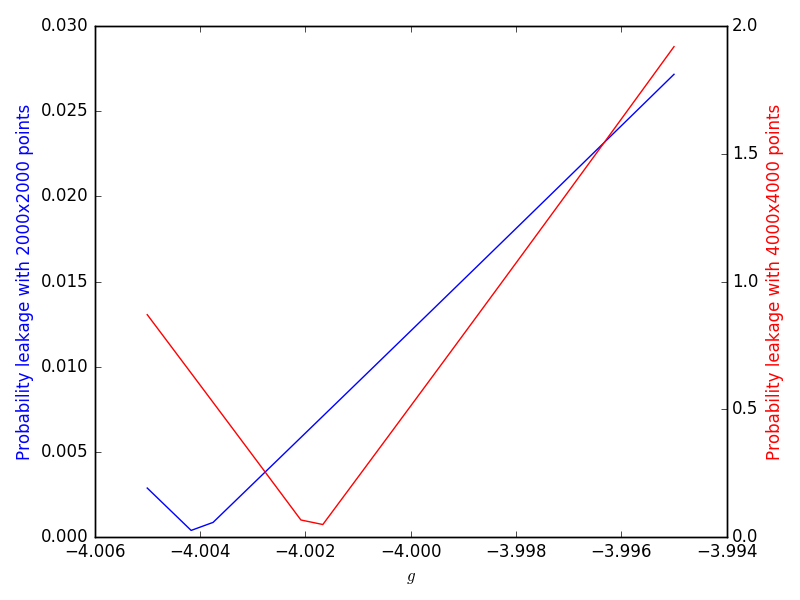
\includegraphics[width=\columnwidth]{errors.png}
\caption{A comparison of the optimal value of $g$, found from the minimum probability leakage, using a discrete space-time grid of 2000x2000 points (blue) compared to 6000x6000 points (magenta). The optimal $g$ value is closer to -4 when space and time more closely approximate a continuum.}
\label{errorsfig}
\end{figure}

As you can see, when the discretisation of space is improved from 2000 points to 6000 points the probability leakage is smaller, for almost every value of $g$ considered. More notably, the interaction parameter with the minimum error in a 2000x2000 box is around $g \approx -4.0025$, whereas for 6000 space points the optimal value is around $g \approx -4.001$. This is significantly closer to the theoretical prediction of -4, agreeing with the hypothesis (see section \ref{Intro}) that the slight disagreement with theory is due to the discretisation of space and possibly time. 


%%%%%%%%%%%%%%%%%%%%%%%%%%%

\section{Results} \label{Results}

\subsection{Collisions}

Two solitons were created at positions symmetric about zero and given equal and opposite velocities to cause them to collide roughly halfway through the time period modelled, as described in section \ref{Methods}. The resulting dynamics were plotted for different values of the interaction parameter $g$, two of which are plotted below (see Fig.\ref{collision}). For small negative values of $g$, the family parameter is small so the solitons are initially fairly diffuse. They therefore produce a large interference pattern when they collide, but emerge with their velocities and relative phase unchanged. Large negative $g$ values and hence very narrow solitons have counterintuitive collision properties, seeming to 'bounce off' one another when in antiphase. This is due to the wave properties of the condensate and is not indicative of the constituent atoms actually undergoing elastic collisions. For relative phases of $\pi/2$ and $3\pi/2$ the interference pattern is asymmetric (see Fig.\ref{asymmetric}), retaining the appearance of solitons bouncing off one another but with one soliton heavily weighted in amplitude. 

\begin{figure*}
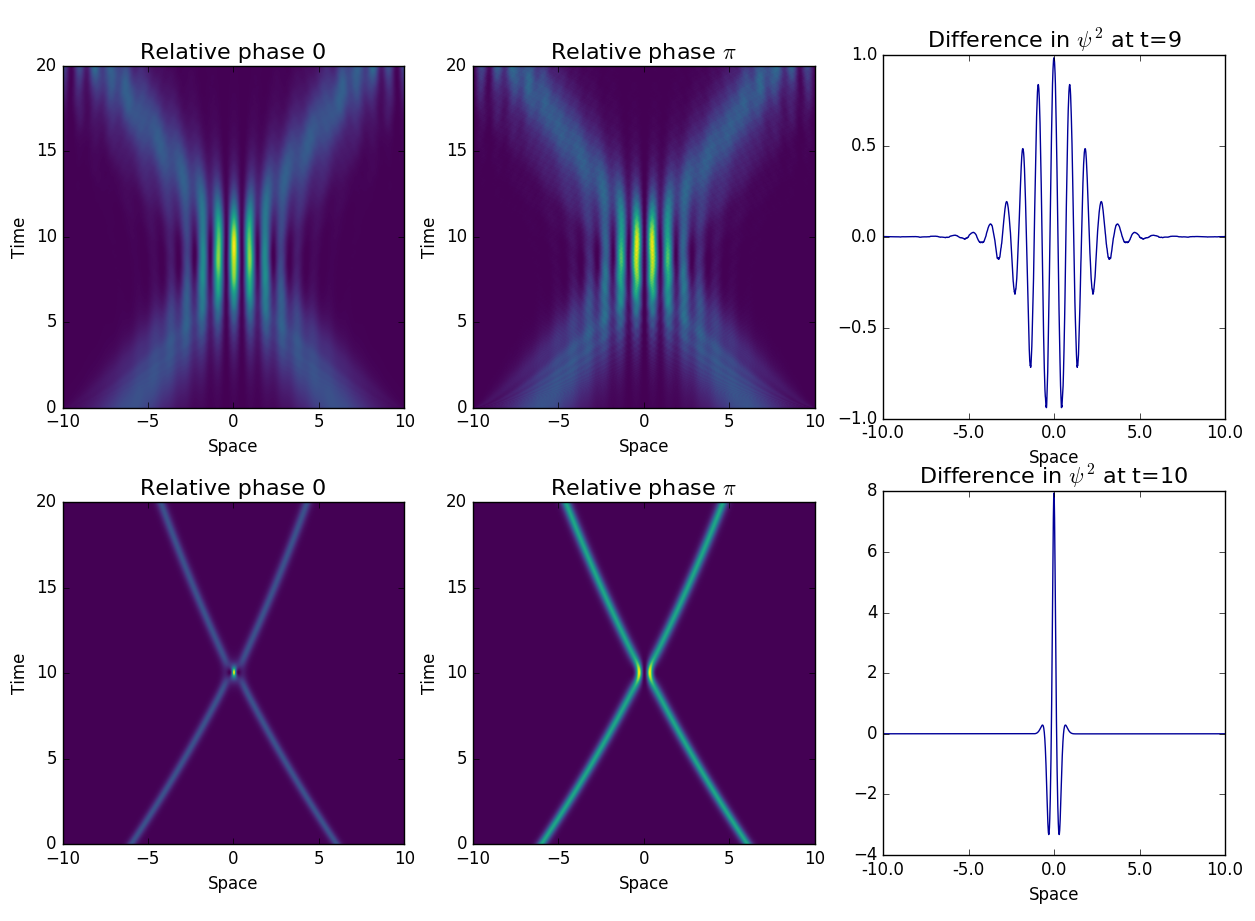
\includegraphics[width=\textwidth]{extensionpic.png}
\caption{A series of graphs showing the collisions of two solitons with speed $|v|=2/3$. Subplots (a)-(c) relate to solitons with $\zeta=0.5$ and subplots (d)-(f) relate to solitons with $\zeta=4$. In plots (a) and (d), the solitons are in phase. In plots (b) and (e) they are in antiphase. Plots (c) and (f) show more clearly the difference between in-phase and antiphase collisions.}
\label{collision}
\end{figure*}

\begin{figure*}
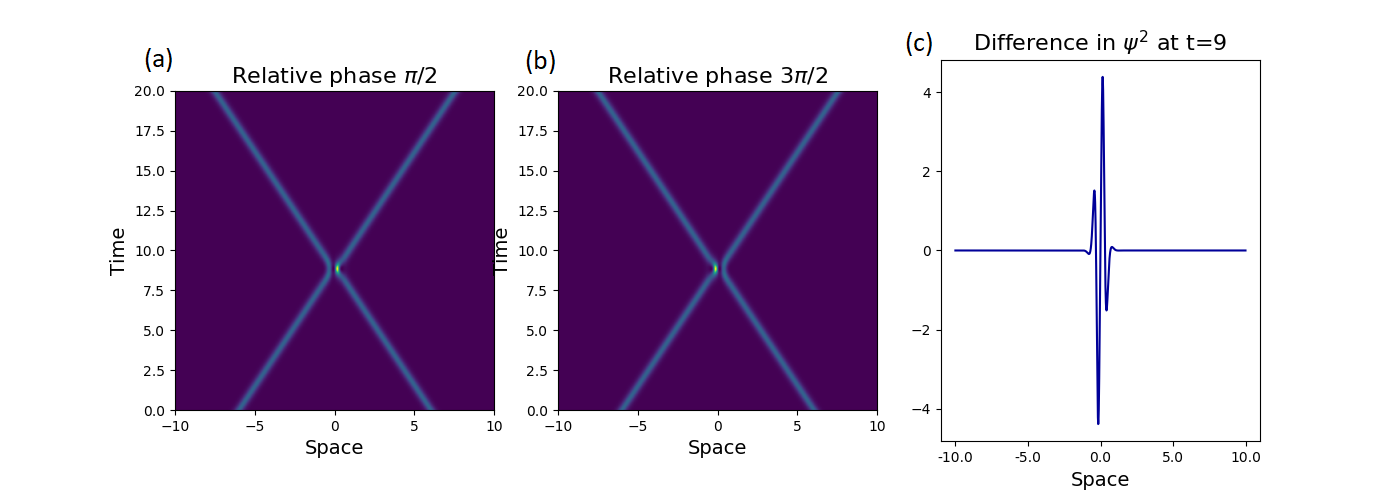
\includegraphics[width=\textwidth]{asymmetrical_collision.png}
\caption{A series of graphs showing the collisions of two solitons with $\zeta=4$ and speed $|v|=2/3$. In subplot (a), the solitons have a relative phase of $\pi/2$. In plot (b) they have a relative phase of $3\pi/2$. Plot (c) shows the difference between these two cases.}
\label{asymmetric}
\end{figure*}

\subsection{Repeated Collisions}


\subsection{Three Solitons}

\begin{figure}[h]
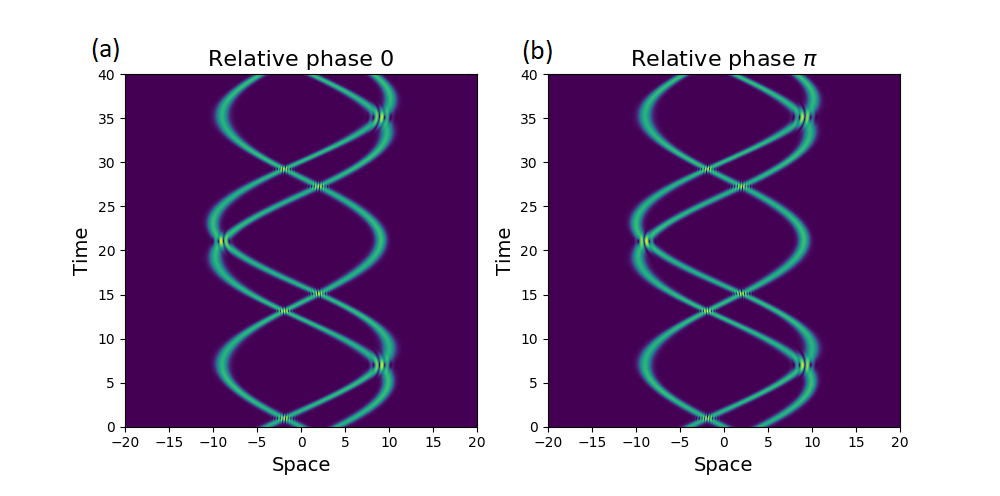
\includegraphics[width=\columnwidth]{3solitons-reg.png}
\caption{Three solitons with equal speeds undergoing collisions with regular (nearly periodic) dynamics. The in-phase and antiphase cases are both shown.}
\end{figure}

\begin{figure}[h]
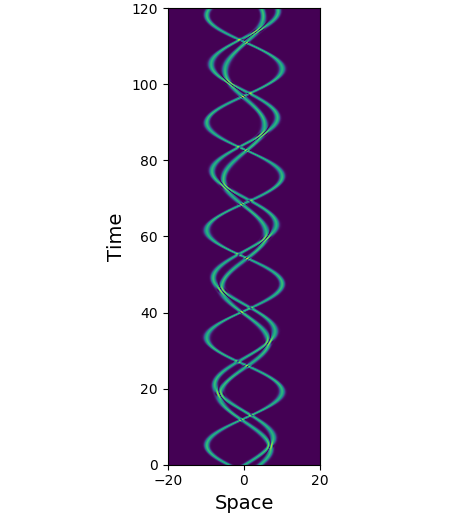
\includegraphics[width=\columnwidth]{chaotic.png}
\caption{Three solitons with speeds 10, $2\pi$ and $3e$ respectively (where $e$ is Euler's number), undergoing collisions with chaotic dynamics.}
\end{figure}

%%%%%%%%%%%%%%%%%%%%%%%%%%%

\section{Discussion} 

\subsection{Collisions}

At first glance, the two phase cases for $\zeta=0.5$ (see Fig.\ref{collision} subplots (a) and (b)) look very similar. In reality, where the solitons are in phase at the time of collision there is a central bright fringe in the interference pattern, as opposed to a central dark fringe in the antiphase case. Subplot (c) is included to illustrate this, showing the difference $\psi_0^2 - \psi_{\pi}^2$ at the time of collision. 

When narrow solitons collide (see Fig.\ref{collision} subplots (d) and (e)), the resulting interference resembles a particle-particle interaction, especially in the antiphase case. However, the strong interactions seem to have caused an attractive force between the solitons as evidenced by the final separation of $\Delta x = 9$ compared to the initial separation of $\Delta x=12$. This result is somewhat unexpected as solitons should not affect each other even under collisions. It is possible that the solitons were not well-separated so formed a short-lived 'bound state' \cite{Bound}.

%%%%%%%%%%%%%%%%%%%%%%%%%%%

\begin{thebibliography}{}

\bibitem{Gross} E. P. Gross (1961), "Structure of a quantised vortex in boson systems", \textit{Il Nuovo Cimento} 				\textbf{20}(3) pp. 454-477. 
\bibitem{Pitaevskii}  L. P. Pitaevskii (1961), "Vortex lines in an imperfect Bose gas", \textit{Sov. Phys. JETP.} \textbf{13}(2) 		pp. 451–454.
\bibitem{Bound} N.-C. Panoiu, I. V. Mel’nikov, D. Mihalache, C. Etrich and F. Lederer (1999), "Multiwavelength pulse 			transmission in an optical fibre - Amplifier system", \textit{Phys. Rev.} \textbf{60}(4868). %bound state
\bibitem{Martin} A. D. Martin, C. S. Adams and S. A. Gardiner (2008), "Bright Solitary-Matter-Wave Collisions in a Harmonic 		Trap: Regimes of Soliton-like Behaviour", \textit{Physical Review A} \textbf{77}(1). %particle model 
\bibitem{Transforms} S. Damgaard Hansen, N. Nygaard and K. Mølmer (2012), "Scattering of matter wave solitons on 			localized potentials", arXiv:1210.1681. %transformations of x, t, psi
\bibitem{Cornish} T. Billam, S. Cornish and S. Gardiner (2010), "Realizing bright matter-wave soliton collisions with 				controlled relative phase", \textit{Physical Review A} \textbf{83}(4). %characteristic soliton lengths 
\bibitem{ExpParams} S. L. Cornish et al. (2009), "Quantum reflection of bright matter-wave solitons", \textit{Physica D} 			\textbf{15}(238), following JILA soliton experiments. 
\bibitem{Feshbach} S. Inouye et al. (1998), "Observation of Feshbach resonances in a Bose–Einstein condensate", 				\textit{Nature} \textbf{392} pp. 151-154. 

\end{thebibliography} 

%%%%%%%%%%%%%%%%%%%%%%%%%%%

\section{Appendix: Code Fragments} \label{Appendix}

The particle model was implented as follows... [include?]

Listings module not working :( 

\end{document}